\documentclass[12pt]{beamer}
\usetheme{Warsaw}
\usepackage[utf8]{inputenc}
\usepackage{amsmath}
\usepackage{amsfonts}
\usepackage{amssymb}
\usepackage{graphicx}
\usepackage{eurosym}
\author{Richard Kwasnicki, Eric Schölzel, Ulrich Huber}
\title{Mining Facebook - Steam Crawling}
%\setbeamercovered{transparent} 
\setbeamertemplate{navigation symbols}{} 
%\logo{\makebox[1\paperwidth]{\includegraphics[width=.5cm,keepaspectratio]{steam.png}}} 
%\institute{} 
%\date{} 
%\subject{} 
\begin{document}



\begin{frame}
\titlepage
%steam logo
\end{frame}


\section{Steam}
%Intro - Steam
\begin{frame}{Steam - Eine Gaming Plattform}
\begin{itemize}
\item Digitale Vertriebsplattform von Valve Corp.
\item Mehr als 125 Mio. "aktive" accounts
\item Rund 12 Mio. Peak am Tag
\item Umsatz in 2015:  3.5 Milliarden Dollar (schätzungsweise 15\% des PC-Spiel Marktes)
\end{itemize}

\end{frame}

\begin{frame}{Warum Steam?}
\begin{itemize}
\item Große Mengen an Daten leicht abgreifbar
\item Umfangreiche API
\item Unter Anderem: Profile, Spiele, Spielzeiten und Freunde abrufbar falls Profil öffentlich 
\end{itemize}
\end{frame}

\begin{frame}{Alle gesammelten Daten}
\begin{itemize}
\item 289.542 Benutzer
\item 260.377 Mit öffentlichem Profil
\item 12.711 Spiele mitsamt Tags
\item 12.684.184 Mio. Spiele von Benutzern
\item 836.467 Freundschaftseinträge (nicht komplett)
%TODO Graphen
%TODO Fun facts avg game time, avg game time 2weeks, 
\end{itemize}
\end{frame}

\begin{frame}{Ziel}
\begin{itemize}
%TODO Bild mit Fragezeichenflagge
%https://upload.wikimedia.org/wikipedia/commons/7/75/Transparent_flag_with_question_mark.png
%Bei länderzzuordnung: fast immer USA obwohl nur 40 Prozent
\item Frage: Lassen sich Benutzer anhand des Spielverhaltens regional zuordnen?
\begin{itemize}
\item Erster Gedanke: Länderzuordnung, aber zu "unsicher", zu viele Länder
\item Einschränkung auf Kontinentzuordnung
\end{itemize}

\end{itemize}
\end{frame}

\section{Daten}
\begin{frame}{Eingesetzte Daten - Allgemein}
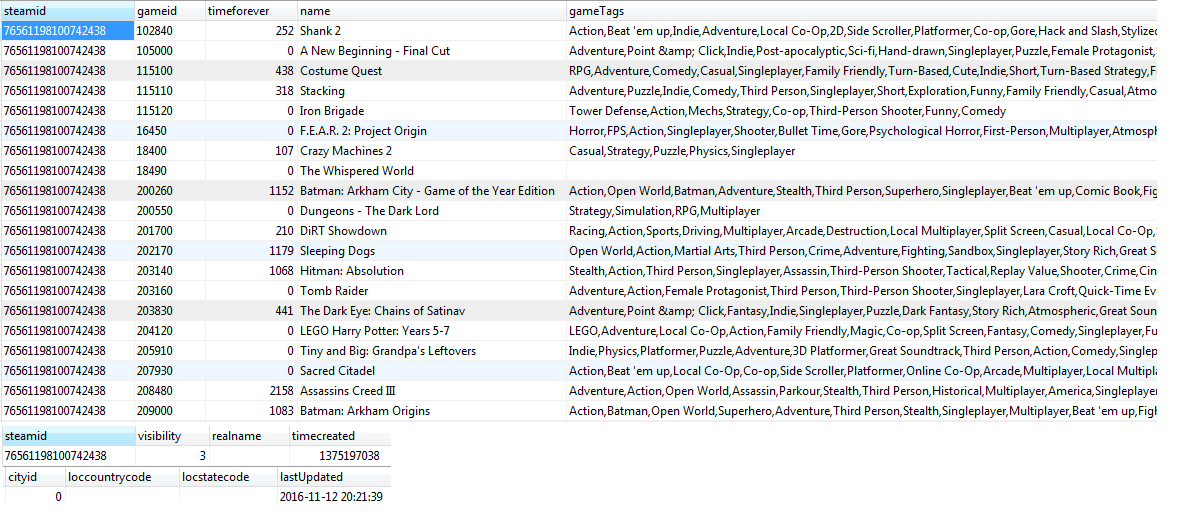
\includegraphics[scale=0.5]{steam_richard_info.png}
\end{frame}

\begin{frame}{Eingesetzte Daten - Aufbereitung}
\begin{itemize}
\item API liefert alle von Nutzern angegebenen Tags zurück $\rightarrow$ möglicherweise zu viele Tags
\item Reduktion notwendig
\item Iteration über alle Spiele, Gruppierung "collapsing" von Tags
\item Beispiel Grand Strategy (weniger) und Strategy (mehr) kommen oft zusammen vor, werden zussamengefasst
%Beispiel CS tausende Tags zu ~10
\end{itemize}

\end{frame}


\begin{frame}{Methoden - Dimensionsreduktion}
\begin{itemize}
%TODO Grafik mit Matrix
\item "Curse of Dimensionality" (\textasciitilde 12.000 Games + \textasciitilde 10.000 Dimensionen durch Gametags und Spielenamen)
\item Lösungsansätze:
\begin{itemize}
\item Reduktion der GameTags (mögliche redundante und unaussagekräftige Tags)
\item TruncatedSVD (PCA)
\end{itemize}
\item Gametagreduktion: Kaum Performancegewinn
\item TruncatedSVD: Leichte Verschlechertung der Genauigkeit (abhängig von Anzahl der Dimensionen), dafür deutlicher Performancegewinn
\end{itemize}
\end{frame}


\section{Ergebnisse}
%\subsection{Welche Klassifikatoren wurden getestet?}
\begin{frame}[fragile]{Welche Klassifikatoren wurden getestet?}
Getestet mit Grid/Randomized Search:
\begin{itemize}
\item SVM 
\item AdaBoost
\item Random Forest
\item KNeighbors
\item Multinomial Naive Bayes
\item SGD
\end{itemize}

Resultat: Alle mit ähnlichen f1-Scores \\
Problem: Teils sehr lange Laufzeiten für einzelne Fits (bspw. 10min bei Random Forest)
\end{frame}

%\subsection{Klassenverteilung}
\begin{frame}[fragile]{Klassenverteilung}
Einfluss ungleichmäßiger Verteilungen auf manche Klassifikatoren: \\
\begin{tabular}{|l|l|l|l|l|l|}
\hline
Real \textbackslash Predicted & Asia & Eu & NA & SA & Summe\\
Asia & \textbf{2} & 129 & 16 & 1 & 148 \\
Europe & 9 & \textbf{1169} & 182 & 12 & 1372 \\
North America & 5 & 462 & \textbf{151} &2 & 620 \\
South America & 3 & 179 & 22 & \textbf{14} & 218 \\
\hline
\end{tabular}
\begin{itemize}
\item Richtig: 1336
\item Falsch: 1022
\item f1-Score: 0,566581849
\item Immer Europa f1-Score: 0,5818490246
\end{itemize}				

\end{frame}

%\subsection{Bestes RF Confusion Matrix Resultat}
\begin{frame}[fragile]{Beste RF Confusion Matrix}
Random Forest, 320 Estimators, ohne PCA/LSA, ohne Scaler \\
Datensatz: 20000 User (5000 pro Kontinent), Spielzeiten, Spielnamen, reduzierte Gametags (21.000 Dimensionen!)\\
\medskip
\begin{tabular}{| l| l| l| l| l|}
\hline
Real \textbackslash Predicted & Asia & Eu & NA & SA \\
Asia & \textbf{236} & 83 & 78 & 90 \\
Europe & 34 & \textbf{262} & 163 & 56 \\
North America & 28 & 96 & \textbf{325} & 29 \\
South America & 99 & 72 & 65 & \textbf{284} \\
\hline
\end{tabular}
\begin{itemize}
\item Richtig: 1107
\item Falsch: 893
\item f1-Score: 0,5535
\item Immer Europa f1-Score: 0,2575
\end{itemize}
\end{frame}

\begin{frame}[fragile]{Overfitting?}
Random Forest, 320 Estimators, Mit LSA (Reduktion auf 10 Dimensionen), ohne Scaler \\
Datensatz: 20000 User (5000 pro Kontinent), Spielnamen, reduzierte Gametags \\
\medskip
\begin{tabular}{| l| l| l| l| l|}
\hline
Real \textbackslash Predicted & Asia & Eu & NA & SA \\
Asia & \textbf{174} & 81 & 74 & 166 \\
Europe & 72 & \textbf{222} & 157 & 83 \\
North America & 52 & 115 & \textbf{252} & 64 \\
South America & 120 & 73 & 61 & \textbf{234} \\
\hline
\end{tabular}
\begin{itemize}
\item Richtig: 882
\item Falsch: 1118
\item f1-Score: 0,441
\item Immer Europa f1-Score: 0,267
\end{itemize}
\end{frame}

%\subsection{Schlussfolgerungen}
\begin{frame}[fragile]{Schlussfolgerungen}
\begin{itemize}
\item f1-Score: 0,5535
\item Immer Europa f1-Score: 0,2575
\end{itemize}
Unsere Pipeline ist mehr als Doppelt so gut wie reines Raten der größten Klasse. \\
$ \rightarrow $ vermutlich Trends erkannt bspw
\begin{itemize}
\item Gesamtspielzeit
\item Beliebte Spiele je Kontinent
\item Anzahl Spiele in Bibliothek
\item Beliebte Genres
\end{itemize}  
\end{frame}

\end{document}